\documentclass[11pt,spanish]{article}
%\usepackage[latin1]{inputenc}
\usepackage[utf8]{inputenc}
%\usepackage[spanish,es-nodecimaldot]{babel}
\usepackage{graphicx}
\usepackage{tikz}
\usepackage{amsmath,amssymb}
%\usepackage{pgf-pie}

\oddsidemargin=0.5cm
\textwidth=16cm
\textheight=48\baselineskip
\topmargin=-1.5cm
\parskip 2truemm
\parindent 0pt
\newcounter{problema}
\typeout{****************************************}
\typeout{****** Configuracion de Guia 11pt ******}
\typeout{****************************************}
%%%%%%%%%%%%%%%%%%%%%%%%%%%%%%%%%%%%%%%%%%%%%%%%%%%%%%%%%%%%%%%%%%%%%%%
\begin{document}
\renewcommand{\labelenumi}{\em \alph{enumi})}
\renewcommand{\labelenumii}{\em \arabic{enumii})}
\newcommand\al{\alpha}
\newcommand\n{\nabla}
\newcommand\F{\vec F}
\newcommand\G{\vec G}
\newcommand\noi{\noindent}
\newcommand\re{\mbox{Re}}
\newcommand\im{\mbox{Im}}
%\newcommand\arg{\mbox{arg}}
\newcommand\Arg{\mbox{Arg}}
\newcommand{\prob}{\stepcounter{problema} \noindent{\bf Problema
\arabic{problema}: }}
\newcommand\pin[2]{\big\langle #1,#2 \big\rangle}

%\input{/home/ortiz/lib/definiciones.tex}
\begin{center}
{\large\sc Facultad de Matem\'atica, Astronom\'ia, F\'isica y Computaci\'on, U.N.C.}

\vspace{2mm}
{\large M\'etodos Matem\'aticos de la F\'isica II}

\vspace{2mm}
{\large Gu\'ia N$^{\sf o}$ 4 (2021)}
\end{center}


\prob{} Calcular las transformadas de Fourier de las siguientes distribuciones:
\begin{enumerate}
\item La distribución de Heaviside (escalón): $\Theta(x-a)$
\item La derivada de la delta de Dirac: $\delta'(x-a)$
\end{enumerate}

\prob{} Considere  el siguiente problema de Neumann en el intervalo $[0,L]$
\[y''=\lambda y\;,\;\; y'(0)=y'(L)=0.
\]

\begin{enumerate}
\item Sin usar la forma expl\'icita de autovalores y autofunciones muestre via el producto escalar:
\[
\langle f,g\rangle := L^{-1} \int^L_0 f(x)g(x) dx\;\;,
\]
que los autovalores son negativos y que las autofunciones a distintos
autovalores son ortogonales respecto del producto escalar.
\item Determine los autovalores y autofunciones.

\end{enumerate}

\prob{}
Resuelva la ecuación de Legendre $ (1-x^2) y'' - 2 x y' + \ell(\ell+1) y = 0$,
donde $\ell(\ell+1)$ es el autovalor. Para ello utilice la solución en forma de
serie de potencias standard
\[
 y = \sum_{n=0}^{\infty} a_n x^{n+s} .
\]
\begin{enumerate}
\item Verifique que la ecuación indicial es $ s(s-1) = 0$.

\item Usando $s=0$ y eligiendo $a_1=0$, obtenga una serie de potencias pares en 
$x$:
\[
 y_{par} = a_0 \left[ 1 - \frac{\ell(\ell+1)}{2!} x^2 + \frac{(\ell-2) \ell (\ell+1)(\ell+3)}{4 
!} x^4 + \ldots \right] .
\]
donde
\[
 a_{j+2} = \frac{j(j+1) - \ell(\ell+1)}{(j+1)(j+2)} a_j .
\]

\item Usando $s=1$ y notando que el coeficiente $a_1$ debe ser nulo, desarrolle 
una serie de potencia impares de $x$:
\[
 y_{impar}= a_0 \left[ x - \frac{(\ell-1)(\ell+2)}{3!} x^3
+ \frac{(\ell-3)(\ell-1) \ell (\ell+2)(\ell+4)}{5!} x^5 + \ldots \right],
\]

donde
\[
a_{j+2} = \frac{(j+1)(j+2) - \ell(\ell+1)}{(j+2)(j+3)} a_j . 
\]

\item Muestre que ambas soluciones, $y_{par}$ y $y_{impar}$, divergen en $x=\pm 1$ 
si la serie es infinita.

\item Finalmente, muestre que eligiendo apropiadamente $\ell$, una de las dos series 
puede ser convertida en un polinomio, avitando así la divergencia.\\

\end{enumerate}


\prob{}
\begin{enumerate}
\item Desarrolle la solución en serie de la ecuación de Hermite $y'' - 2x y' + 2 \alpha y = 0$, donde $\alpha$ es el el autovalor. Verifique que la 
ecuación indicial es $s(s-1) = 0$ (como en el Problema anterior). De la misma 
forma que en el problema anterior encuentre para $s=0$ y $s=1$ relaciones de 
recurrencia para los coeficientes de la serie de tal forma que
\[
 s= 0 , \quad a_{j+2} \propto a_j, \; \mbox{con} \; j  \; \mbox{par}, \quad 
y_{par} = a_0 \left[ 1 + \ldots\right] ,
\]
mientras que

\[
 s= 1 , \quad a_{j+2} \propto a_j, \; \mbox{con} \; j  \; \mbox{par}, \quad 
y_{impar} = a_1 \left[ 1 + \ldots\right] .
\]

\item Muestre que ambas soluciones en forma de serie son convergentes para todo 
$x$, y que el cociente de coeficientes sucesivos se comporta, para índices 
grandes, como el cociente de los coeficientes de la expansión en serie de la 
función $\exp(-x^2)$.

\item Muestre que eligiendo apropiadamente el parámetro $\alpha$, la solución en 
seire puede ser truncada y conertida en polinomios finitos. Estos polinomios 
son los polinomios de Hermite.\\
\end{enumerate}

\prob{}
Un conjunto de funciones $u_n(x)$ satisfacen la ecuación de Sturm-Liouville
\[
 \frac{d}{dx}\left[ p(x) \frac{d}{dx} u_n(x) \right] + \lambda_n u_n(x) = 0.
\]

Las funciones $u_m$ y $u_n$ satisfacen condiciones de contorno que llevan a la 
ortogonalidad. Los correspondientes autovalores $\lambda_m$ y $\lambda_n$ son 
distintos. Pruebe que, con condiciones de contorno apropiadas, $u'_m(x)$ y 
$u'_n(x)$ son ortogonales con función de peso $p(x)$.\\


\prob{} Resuelva, usando el método de las características, los siguientes problemas escalares
de primer orden
\begin{enumerate}

\item $\cfrac{1}{x} \cfrac{\partial u}{\partial x} + \cfrac{\partial u}{\partial y}=0,  \hspace{1cm} x>0,  \hspace{1cm} u(x,0)=g(x).  
$
\item $ x\cfrac{\partial u}{\partial x} - 2y\cfrac{\partial u}{\partial y} = 0, \qquad u(1,y) = 1+2y$.

\item $x \cfrac{\partial u}{\partial x} - 2y \cfrac{\partial u}{\partial y}= u^2, \,\,\,\, u(x,0)=x^3.$

\item $y\cfrac{\partial u}{\partial x} - x\cfrac{\partial u}{\partial y} = e^u, \qquad u(0,y) = y^2-1$.

\end{enumerate}

\prob{} Resuelva la ecuación de Laplace dentro de un rect\'angulo de lados  $a$ y $b$ con las condiciones de borde dadas. 


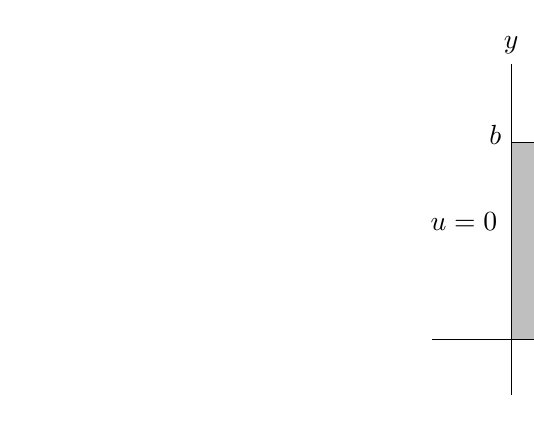
\begin{tikzpicture}[scale=1]
\hspace{5cm}
\begin{scope}
\draw[fill=lightgray] (0,0) rectangle (3.5,2.5);
\end{scope}
\draw (-1,0)--(4,0) node[right]{$x$};
\draw (0,-0.7)--(0,3.5) node[above]{$y$};
\node at (1.8,1.3) {$\Delta u=0$};
\node at (3.6,-0.2) {$a$};
\node at (-0.2,2.6) {$b$};
\node at (4.3,1.5) { $u=2y$}; 
\node at (1.8,2.8) {$u=x$}; 
\node at (1.6,-0.3) {$u=0$};
\node at (-0.6,1.5) {$u=0$};
\end{tikzpicture}

\prob{}
Resuelva la ecuaci\'on de Laplace dentro de una regi\'on rectangular $0 \leq x \leq L, 0 \leq y \leq H$, con las siguientes condiciones de borde:

 $\frac{\partial u}{\partial x}(0,y)=0, \hspace{1cm} u(L,y)=2y, \hspace{1cm} u(x,0)=0, \hspace{1cm} u(x,H)=0$

\prob{} Resuleva la ecuaci\'on $\Delta u=1$ dentro del rect\'angulo de lados $a$ y $b$ con la condici\'on $u=0$ en los cuatro lados.





\prob{} Resuelva la ecuación de Laplace en el interior de un paralelepípedo definido por los planos $x=0, x=c, y=0, y=c, z=0, z=L$ tal que $\psi=0$ en todas sus caras excepto en $z=L$ donde $\psi=V_o$.

\prob{} Considere la región en el plano $xy$ delimitada por $0 \leq x \leq a,
0 \leq y < \infty$. Encuentre la solución de la ecuación $\Delta \psi =0 $ en dicha región con las condiciones: $\psi(0,y)=0, \psi(a,y)=0, \psi(x,0)=A(1-\frac{x}{a})$, donde $A$ es una constante.

\prob{}
Encuentre la soluci\'on acotada de la ecuaci\'on $\Delta u=0$ en el exterior de un disco de radio $a$ sujeto a las condiciones de borde $u(a,\theta)= \ln 2 + 4 \cos(3\theta)$.

\prob{} 
Encuentre aquella soluci\'on de la ecuaci\'on de Laplace en el  interior del disco unitario de radio $r=1$ que tenga valores en la frontera dados por $$f(1, \phi)=\begin{cases} 
      V_o               & 0<\phi<\pi \\
      0,  & \pi<\phi<2 \pi 
      \end{cases}$$
donde $V_o$ es una constante.


\prob{} Considere dos cilindros coaxiales conductores de longitud infinita de radios $a$ (interior) y $b$ (exterior). El potencial se fija de tal manera que $V(r=a)=V_o$ y $V(r=b)=-V_o$. Sabiendo que el potencial electrostático, en una región libre de cargas, satisface la ecuación de Laplace, calcule el potencial en las regiones:

a) $r < a$

b) $a <r < b$

c) $b < r$

\prob{}  Obtenga la temperatura, $T$, del estado estacionario (es decir $\Delta T=0$) en el interior de un tubo cilíndrico recto finito de longitud $L$ y radio $a$. El tubo se mantiene a temperatura $T=0$  en las superficies $r=a$ y $z=0$, mientras que en $z=L$ se mantiene a una temperatura $T(r,\phi , L)=T_o f(r,\phi)$. Aqu\'{\i}, $(r,\phi , z)$ son las coordenadas cil\'{\i}ndricas naturales. Particularice la solución para $f(r, \phi)=r \sin \phi$.

  
\prob{} Un cilindro recto s\'olido semi-infinito de radio $a$ mantiene su superficie curva a temperatura $T=0$ y su base a $T_o$. Encuentre la distribuci\'on de temperatura en el cilindro en el estado estacionario.  

\prob{} Considere una esfera metálica de radio unitario, con una condición de frontera:
$$U(1, \theta)=\begin{cases}  
      U_o               & 0<\theta<\pi/2 \\
      0,  & \pi/2<\theta<\pi 
      \end{cases},$$ donde $U_o$ es una constante. 
Podemos dar a este problema, las siguientes interpretaciones (entre otras), para las cuales nos interesa conocer su  solución:
\begin{enumerate}
\item Suponga que la esfera es sólida y la condición de frontera representa una distribución de temperatura. Determine el estado estacionario.
\item Suponga que la esfera es hueca y la condición de frontera representa una distribución de potencial electrostático. Encuentre el valor del potencial dentro y fuera de la esfera.
\end{enumerate}


\end{document}


